%% Context-Conditional, Cost-Asymmetric Bandwidth Allocation
%% IEEEtran conference template (ICCIT / TENCON / WCNC-workshop tier).
%% Build:  pdflatex paper && bibtex paper && pdflatex paper && pdflatex paper
%% Every number here is produced by the scripts in ../../experiments/ and read
%% from ../../experiments/results/. Nothing is transcribed by hand.

\documentclass[conference]{IEEEtran}
\IEEEoverridecommandlockouts

\usepackage{cite}
\usepackage{amsmath,amssymb,amsfonts}
\usepackage{graphicx}
\usepackage{booktabs}
\usepackage{url}
\usepackage{textcomp}

\graphicspath{{../figures/}}

\newcommand{\gpx}{GP}
\newcommand{\robix}{Robi}

\begin{document}

\title{Context-Conditional, Cost-Asymmetric Bandwidth\\ Allocation from Sparse, Irregularly Sampled\\ Operator Traces}

\author{\IEEEauthorblockN{[Author name]}
\IEEEauthorblockA{\textit{Department of Electrical and Electronic Engineering} \\
\textit{Bangladesh University of Engineering and Technology}\\
Dhaka, Bangladesh \\
2106110@eee.buet.ac.bd}
}

\maketitle

\begin{abstract}
Cellular capacity planning is usually studied as a forecasting problem and scored by
RMSE. We argue this is the wrong target twice over: the decision an operator makes is
an \emph{allocation}, whose costs are asymmetric, and it must be made at a \emph{lead
time}, not one step ahead with the previous measurement in hand. Working from two
$\sim$900-sample traces from Dhaka cell sites, we first show that the sampling rate of
both is misread by the standard treatment: neither is hourly (86 and 99 minutes per
sample), so a 24-sample ``daily'' lag spans 34.4 and 39.6 hours and correlates
\emph{negatively} with demand. We rebuild the evaluation protocol around the measured
sampling rate, with leak-safe features, rolling-origin folds, naive baselines and
Diebold--Mariano tests. We then add lead time and an allocation layer: with an
asymmetric cost ratio $\kappa$, the cost-minimising allocation is the $\tau$-quantile
of the predictive distribution with $\tau^{*}=\kappa/(1+\kappa)$, calibrated
conformally. The advantage of a learned model over a naive forecaster \emph{at the same
lead} grows from 14\% at one step to 59\% at 11.5 hours. Our central contribution is
that this calibration must be \textbf{context-conditional}: auditing the traces'
hand-labelled flags shows most do not predict the \emph{level} of demand---including
the weekend flag both source files are named after ($p=0.77$)---but rainfall raises
residual $\sigma$ by 33\% ($p<0.001$). Context acts on variance, not level. A
marginally calibrated allocator consequently meets its 95\% target overall while
delivering 86.6\% [.807,\,.912] during elevated-risk periods. At the operator's own
cost ratio, context-adaptive calibration provisions 7.5\% (\gpx) and 14.8\% (\robix)
more cheaply than a fixed-margin rule tuned with hindsight. We report two negative
results in full: correcting the feature design does not improve RMSE, and
split-conformal coverage fails a $\pm 2\%$ check on real data (2 of 30 configurations
pass) because exchangeability breaks under drift. Online conformal calibration repairs
it completely, passing 30 of 30 at lead times from 1.4 to 24 hours on both operators.
\end{abstract}

\begin{IEEEkeywords}
bandwidth allocation, cellular traffic prediction, conformal prediction, irregular
sampling, cost-asymmetric optimisation, service-level agreements
\end{IEEEkeywords}

\section{Introduction}

Mobile operators provision capacity against demand they cannot observe yet. The applied
literature treats this as a forecasting problem: assemble lag features, train a set of
models---gradient boosting, ARIMA, an LSTM---and rank them by RMSE on a held-out split.
The ranking is then reported as though the best-ranked model were the best
\emph{system}. Three things go wrong in that framing, and they compound.

\textbf{The objective is not symmetric.} Under-provisioning breaches a service-level
agreement and degrades quality of experience; over-provisioning wastes capital. These
costs differ by a factor of 5--20 in practice, and a loss function penalising them
equally optimises for neither. The decision an operator actually makes is an
allocation, and the cost-minimising allocation is a \emph{quantile} of the predictive
distribution rather than its mean---which changes the model class, the loss and the
evaluation metric together.

\textbf{The horizon is not one step.} Reported evaluations almost universally predict
$y_t$ given $y_{t-1}$, feeding true lagged values at every step. No provisioning
decision can be made that way: capacity for an interval is committed before that
interval's predecessor has been measured. This matters more than it appears, and in a
direction that is not obvious. We find that at one step a learned model beats a
one-line persistence baseline by 14\%---a margin thin enough to invite the conclusion
that the modelling is not worth its complexity---but that at an 11.5-hour lead the same
model beats the naive forecaster \emph{at that same lead} by 59\%. The one-step
protocol systematically understates the value of learning, because it is precisely the
regime in which the trivial baseline is strongest.

\textbf{The evaluation inherits assumptions from the data format.} Operator traces are
frequently irregularly sampled, and a design matrix indexed by sample count silently
encodes a sampling rate that may be wrong. Neither trace studied here is hourly (86 and
99 minutes per sample), so the lag of 24 samples used throughout as the ``daily'' lag
spans 34.4 and 39.6 hours and correlates \emph{negatively} with demand. Every seasonal
statement---STL decomposition, ACF peak, \texttt{ARIMA(24,1,0)}---is then made on the
wrong time axis.

We address all three on two $\sim$900-sample traces from Dhaka cell sites. The small
sample is a genuine constraint and we do not pretend otherwise; it is also why the
methods chosen here are the right ones. Conformal calibration is distribution-free and
finite-sample valid, so it needs no parametric error model that 900 points cannot
support, and an explicit estimability guard makes the sample-size ceiling visible
rather than letting it be silently exceeded.

Our central observation concerns the hand-labelled contextual annotation these traces
carry---rainfall, political gatherings, power cuts, promotional offers. Such annotation
for a specific Dhaka cell site cannot be downloaded, and it is the dataset's
distinctive asset; it is also, in the standard treatment, fed to models as binary
dummies and never validated. Validating it shows that most flags do not predict the
\emph{level} of demand at all, including the weekend flag both source files are named
after. What rainfall predicts is \emph{dispersion}: residual $\sigma$ rises 33\%.
Context acts on variance, not mean---and a point forecaster with a context dummy
structurally cannot express that, while a context-conditional prediction interval can.
This converts weak mean-predictors into useful risk signals, which is the right use of
annotation that is sparse, hand-made and noisy.

\textbf{Contributions.}
\begin{enumerate}
\item A sampling-aware, leak-safe evaluation protocol for irregularly sampled operator
traces, in which every seasonal hyperparameter is \emph{derived} from the measured
sampling rate rather than assumed (Section~\ref{sec:protocol}).
\item A multi-horizon evaluation showing that the value of learned forecasting on these
traces is concentrated at operationally relevant lead times and is nearly invisible at
one step (Section~\ref{sec:lead}).
\item A cost-asymmetric allocation layer with conformal calibration, evaluated on
provisioning cost rather than forecast error (Section~\ref{sec:alloc}).
\item \textbf{Context-conditional calibration}: the observation that hand-labelled
context acts on the \emph{variance} of demand rather than its level, the demonstration
that marginal calibration therefore fails inside high-risk contexts, and the repair
(Section~\ref{sec:context}).
\item A cold-start transfer study (Section~\ref{sec:coldstart}) and a zero-shot
foundation-model comparison showing that the sampling-rate measurement predicts, in
advance, whether such a model will work at all (Section~\ref{sec:zeroshot}).
\end{enumerate}

\section{Related Work}

\textbf{Cellular traffic prediction.} The applied literature on mobile traffic
forecasting is large and well surveyed~\cite{wang2024survey}. Its dominant shape is the
one we depart from: assemble lag and calendar features, train a panel of models, and
rank them by RMSE or MAPE on a held-out split. Three assumptions ride along unexamined:
that the loss is symmetric, that one-step-ahead error is the operational quantity, and
that the sampling grid is whatever the column index implies. This paper argues all
three matter, and demonstrates that the third is measurable rather than rhetorical.

\textbf{SLA-aware prediction and slice resource allocation.} Closest to our framing is
the work of Tuna and Soysal~\cite{tuna2023multivariate,tuna2023spatiotemporal}, which
predicts NextG slice traffic under explicit SLA violation constraints rather than under
squared error, and observes---as we do---that a symmetric loss is the wrong objective
when breaching a service level and wasting capacity cost different amounts.
MicroOpt~\cite{sulaiman2024microopt} goes further into the decision layer, optimising
slice resources against a learned model of SLA satisfaction. We differ in three ways.
Those systems train an asymmetric or constrained \emph{point} predictor; we keep an
ordinary point model and move the asymmetry into a calibrated quantile, which decouples
the forecaster from the cost ratio and lets $\kappa$ change without retraining. Their
guarantees are empirical over large regularly sampled datasets; ours are
distribution-free and finite-sample, which is what $\sim$900 irregularly sampled points
can actually support. And neither conditions the service level on operating context,
which is our central contribution.

\textbf{Conformal prediction.} We build directly on the conformal
framework~\cite{vovk2005algorithmic,angelopoulos2024foundations}: given exchangeable
residuals, a calibration quantile yields finite-sample marginal coverage with no
distributional assumption. Conformalized quantile regression~\cite{romano2019cqr} makes
interval width respond to local difficulty, and Mondrian conformal prediction
partitions the calibration set into groups to obtain per-group validity. Exact
conditional coverage is impossible without assumptions, and Gibbs, Cherian and
Cand\`{e}s~\cite{gibbs2023conditional} characterise what is achievable against a
specified class of shifts. Section~\ref{sec:context} is an applied instance of that
tension: the groups are not statistical constructs but hand-labelled operating
conditions---rainfall, power cuts---and the finding is that a marginally valid
allocator is systematically invalid inside the group where the network is most
stressed. Separately, exchangeability itself fails on a drifting two-month trace;
adaptive conformal inference~\cite{gibbs2021adaptive} updates the requested level
online from realised breaches and restores long-run coverage without assuming
exchangeability at all.

\textbf{Time-series foundation models.} Chronos~\cite{ansari2024chronos} tokenises
scaled time-series values and trains a language-model architecture over them;
TimesFM~\cite{das2023decoder} is a decoder-only model pretrained on a large corpus.
Both are marketed on zero-shot transfer to unseen series. Neither consumes
timestamps---they read a bare sequence of values---which is inconsequential on a
regular grid and, we show in Section~\ref{sec:zeroshot}, decisive on an irregular one.
We are not aware of prior work linking zero-shot foundation-model performance to the
misregistration between a trace's sampling interval and its dominant period, and we
offer that as a cheap pre-deployment diagnostic.

\textbf{Evaluation methodology.} Our protocol follows standard forecasting practice
that the applied cellular literature frequently omits: rolling-origin evaluation rather
than a single split~\cite{tashman2000outofsample}, scale-free error reporting against a
naive baseline~\cite{hyndman2006another}, and Diebold--Mariano
tests~\cite{diebold1995comparing} with Benjamini--Hochberg false-discovery
control~\cite{benjamini1995controlling} when ranking a panel of models. None of this is
novel. It is included because applying it to these traces reverses several published
conclusions.

\section{Data}

\begin{table}[htbp]
\caption{The two operator traces.}
\label{tab:data}
\centering
\begin{tabular}{lcc}
\toprule
& \textbf{Grameenphone} & \textbf{Robi Dhaka-3} \\
\midrule
Observations & 905 & 888 \\
Span (days) & 55 & 62 \\
Median sampling interval & \textbf{86 min} & \textbf{99 min} \\
Samples per day & $\sim$17 & $\sim$15 \\
Mean demand & 92.9 Gbps & 145.5 Gbps \\
Contextual flags & 9 & 5 \\
\bottomrule
\end{tabular}
\end{table}

Both traces carry hand-annotated local context (\texttt{is\_rain},
\texttt{is\_political\_gathering}, \texttt{is\_offer}, \texttt{is\_powercut},
\texttt{is\_drama}, and others). This annotation is the distinctive asset of the
dataset---it is not something that can be downloaded for a Dhaka cell site---and
Section~\ref{sec:context} is built on it.

\section{A Corrected Evaluation Protocol}
\label{sec:protocol}

\subsection{The traces are not hourly}
\label{sec:nothourly}

Both traces are treated as hourly in the standard treatment, so a lag of 24 samples is
used as the daily lag. At 86 min per sample that lag spans 34.4 hours and sits roughly
anti-phase to the daily cycle.

\begin{table}[htbp]
\caption{Autocorrelation at the measured daily period versus at lag 24, and the
seasonal-naive RMSE penalty for using the latter.}
\label{tab:acf}
\centering
\begin{tabular}{lcc}
\toprule
& \textbf{Measured period} & \textbf{At lag 24} \\
\midrule
\multicolumn{3}{l}{\emph{Autocorrelation}} \\
\gpx\ (period 17) & \textbf{+0.451} & $-0.347$ \\
\robix\ (period 15) & \textbf{+0.822} & $-0.383$ \\
\midrule
\multicolumn{3}{l}{\emph{Seasonal-naive RMSE (penalty)}} \\
\gpx & 18.16 & 28.42 \ (+56\%) \\
\robix & 26.58 & 74.12 \ (\textbf{+179\%}) \\
\bottomrule
\end{tabular}
\end{table}

\begin{figure}[htbp]
\centering
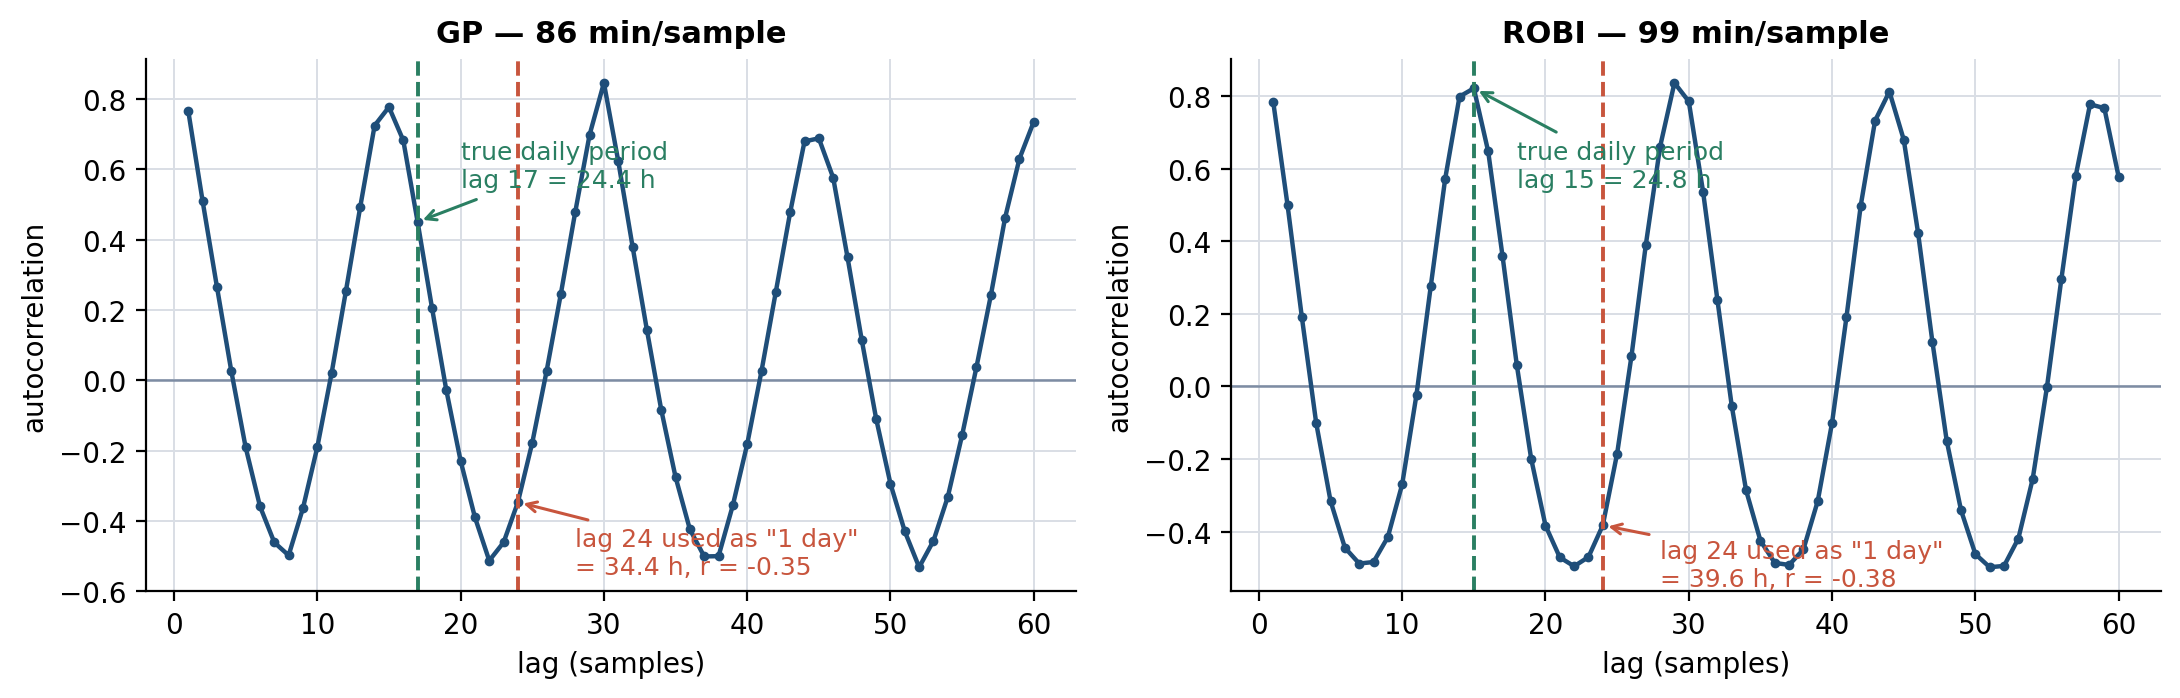
\includegraphics[width=\columnwidth]{fig1_autocorrelation.png}
\caption{Autocorrelation by lag, with the measured daily period and lag 24 marked. The
feature used throughout the standard treatment as the daily lag correlates negatively
with demand on both traces.}
\label{fig:acf}
\end{figure}

Every seasonal statement made on the sample-count axis---STL decompositions, ACF and
FFT peaks, \texttt{AutoReg(lags=24)}, \texttt{ARIMA(24,1,0)},
\texttt{ExponentialSmoothing(seasonal\_periods=24)}---is stated on the wrong axis. In
this work the daily period is measured per operator and every seasonal hyperparameter
derives from it, while seasonality itself is carried by Fourier terms in wall-clock
time, which are exact under irregular sampling.

\subsection{Target leakage}

Rolling statistics computed without a preceding shift place $y_t$ inside its own
feature vector. Restoring the shift moves the best \gpx\ result from 6.54 to 19.30 RMSE
($+195$\%) and \robix\ from 16.32 to 27.37 ($+68$\%). The corrected \gpx\ figure is
worse than predicting the training mean (18.87). We enforce this structurally:
\texttt{assert\_no\_leakage} perturbs the final target value and asserts that no
feature column moves, and the benchmark refuses to run if it fails.

\subsection{Baselines, folds, and significance}

All models share one rolling-origin fold schedule (8 expanding-window folds), every
table reports naive baselines (persistence, seasonal-naive at the measured period,
drift, train-mean) and MASE alongside RMSE, and rankings carry Diebold--Mariano
$p$-values under Benjamini--Hochberg correction.

\begin{table}[htbp]
\caption{Corrected one-step benchmark (RMSE, mean $\pm$ sd across 8 folds).}
\label{tab:benchmark}
\centering
\begin{tabular}{lcc}
\toprule
\textbf{Model} & \textbf{\gpx} & \textbf{\robix} \\
\midrule
Random forest & \textbf{10.41 $\pm$ 1.19} & \textbf{20.75 $\pm$ 4.42} \\
XGBoost & 10.80 & 21.32 \\
Ridge & 11.26 & 22.72 \\
\textbf{Persistence} & \textbf{12.13} & \textbf{29.75} \\
Seasonal-naive (measured) & 18.31 & 26.26 \\
Seasonal-naive at lag 24 & 29.74 & 73.51 \\
\bottomrule
\end{tabular}
\end{table}

\begin{figure}[htbp]
\centering
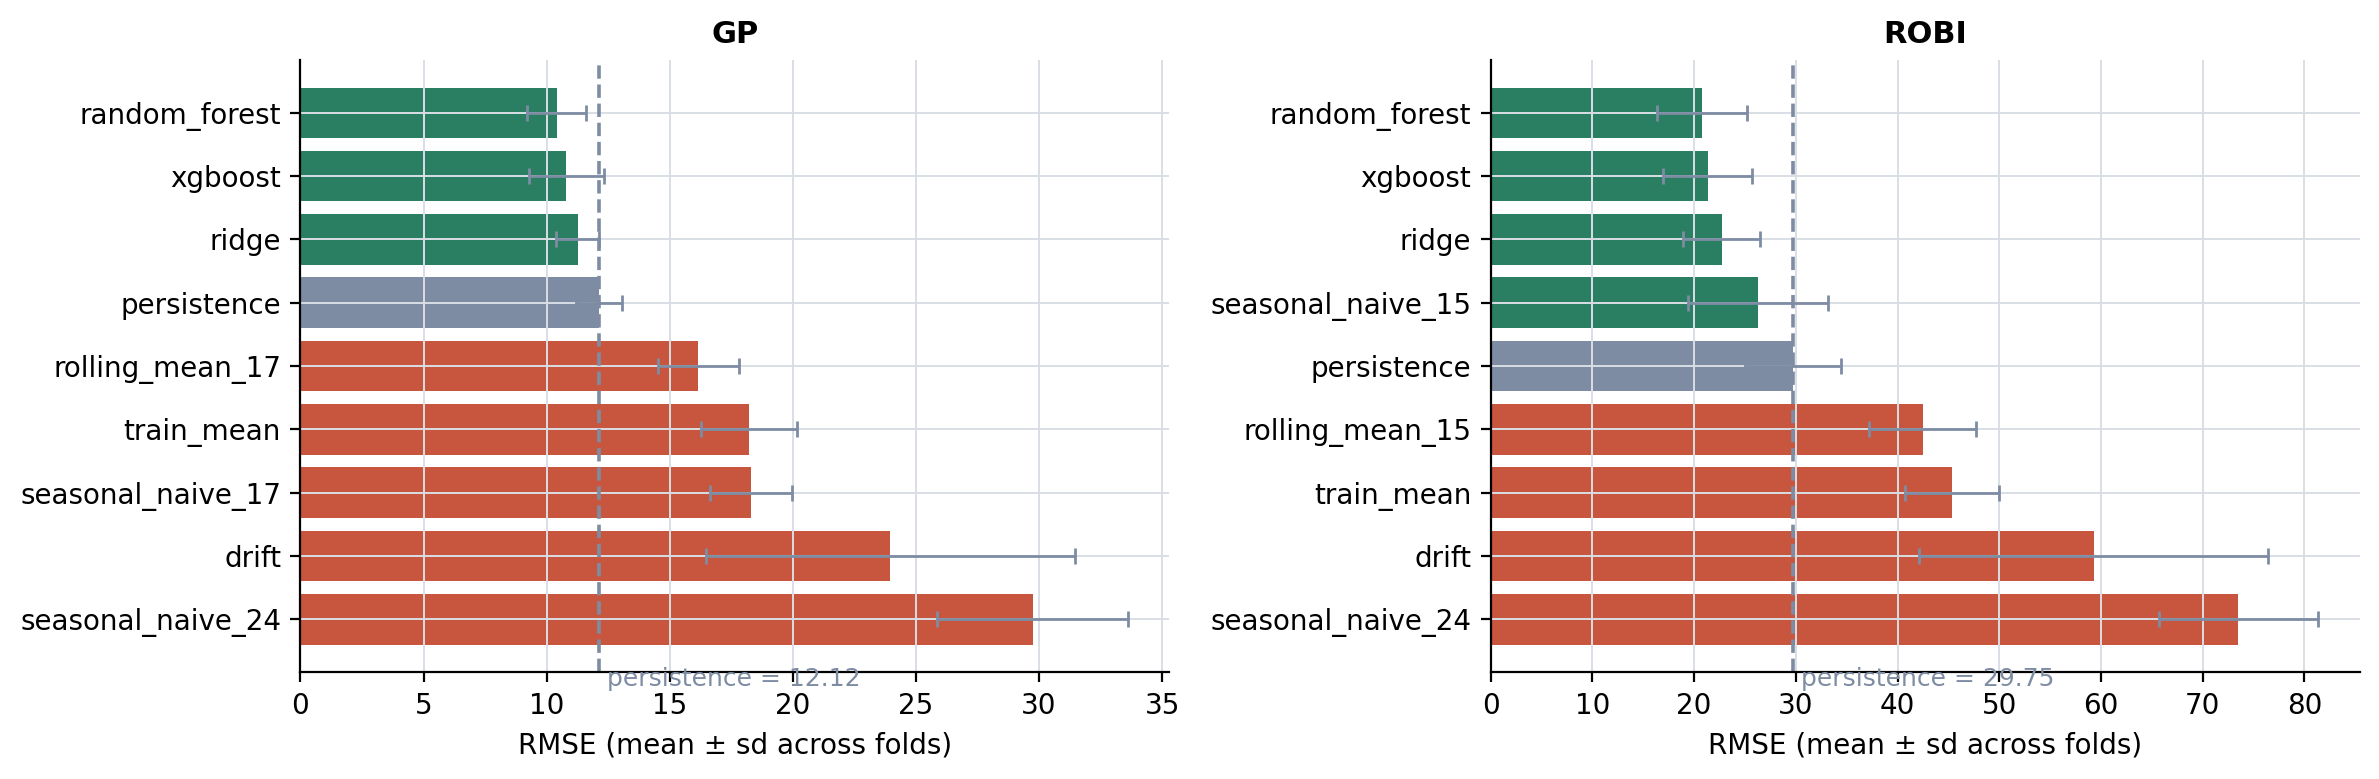
\includegraphics[width=\columnwidth]{fig2_benchmark.png}
\caption{Corrected benchmark with fold spreads and the persistence line.}
\label{fig:benchmark}
\end{figure}

\subsection{A negative result: the correction does not improve accuracy}
\label{sec:ablation}

The feature ablation is reported in full because it cuts against the correction. On
both operators, a faithful reproduction of the original feature design (with the leak
removed) is within noise of, and on \robix\ slightly better than, the corrected design.

\begin{table}[htbp]
\caption{Feature ablation (RMSE). The corrected design does not win.}
\label{tab:ablation}
\centering
\begin{tabular}{lcc}
\toprule
\textbf{Configuration} & \textbf{\gpx} & \textbf{\robix} \\
\midrule
Lags only & 9.98 & 21.78 \\
Original design (leak removed) & 10.11 & \textbf{20.53} \\
Original design, lag corrected & 10.12 & 21.39 \\
Full corrected design & 10.41 & 20.75 \\
\bottomrule
\end{tabular}
\end{table}

Tree ensembles route around a mis-specified \texttt{lag\_24} by leaning on the short
lags, so the sampling-rate error costs almost nothing in RMSE. Its cost is
\textbf{interpretive}: every seasonal claim in the standard treatment is stated on the
wrong axis, and Section~\ref{sec:nothourly} shows what the error costs a model that
cannot route around it. We report this rather than bury it.

\section{Lead Time}
\label{sec:lead}

Every result above, and every result in the studies this extends, predicts $y_t$ with
$y_{t-1}$ in hand. No network provisions from that: the capacity decision for an
interval is made before the previous measurement arrives.

We evaluate direct multi-horizon models at 1.5--24\,h. Three details make the
evaluation honest.

\textbf{Feature roles.} History columns (lags, rolling statistics) are read at the
forecast \emph{origin}; Fourier and calendar terms, being deterministic functions of
wall-clock time, are read at the \emph{target}. An operator provisioning for 9\,p.m.
knows it will be 9\,p.m.

\textbf{Per-horizon baselines.} An $h$-step model is scored against an $h$-step naive
forecaster. Comparing a 24-hour-ahead model to one-step persistence is how multi-step
results are most often overstated.

\textbf{Embargo.} Direct training pairs carry targets $h-1$ rows after their origin, so
those rows are dropped from fitting and calibration; otherwise the model is trained on
outcomes that had not occurred when the first test forecast was issued.

\begin{table}[htbp]
\caption{\gpx: RMSE against forecast lead time, 8 folds.}
\label{tab:horizon}
\centering
\setlength{\tabcolsep}{4pt}
\begin{tabular}{lccccc}
\toprule
\textbf{Lead} & 1.43\,h & 2.87\,h & 5.73\,h & 11.47\,h & 24.37\,h \\
\midrule
Random forest & 10.40 & 11.85 & 12.48 & 12.83 & 12.82 \\
Naive at lead & 12.12 & 17.41 & 25.11 & 31.16 & 18.26 \\
\textbf{Advantage} & $\mathbf{-14\%}$ & $\mathbf{-32\%}$ & $\mathbf{-50\%}$ & $\mathbf{-59\%}$ & $\mathbf{-30\%}$ \\
\bottomrule
\end{tabular}
\end{table}

\begin{figure}[htbp]
\centering
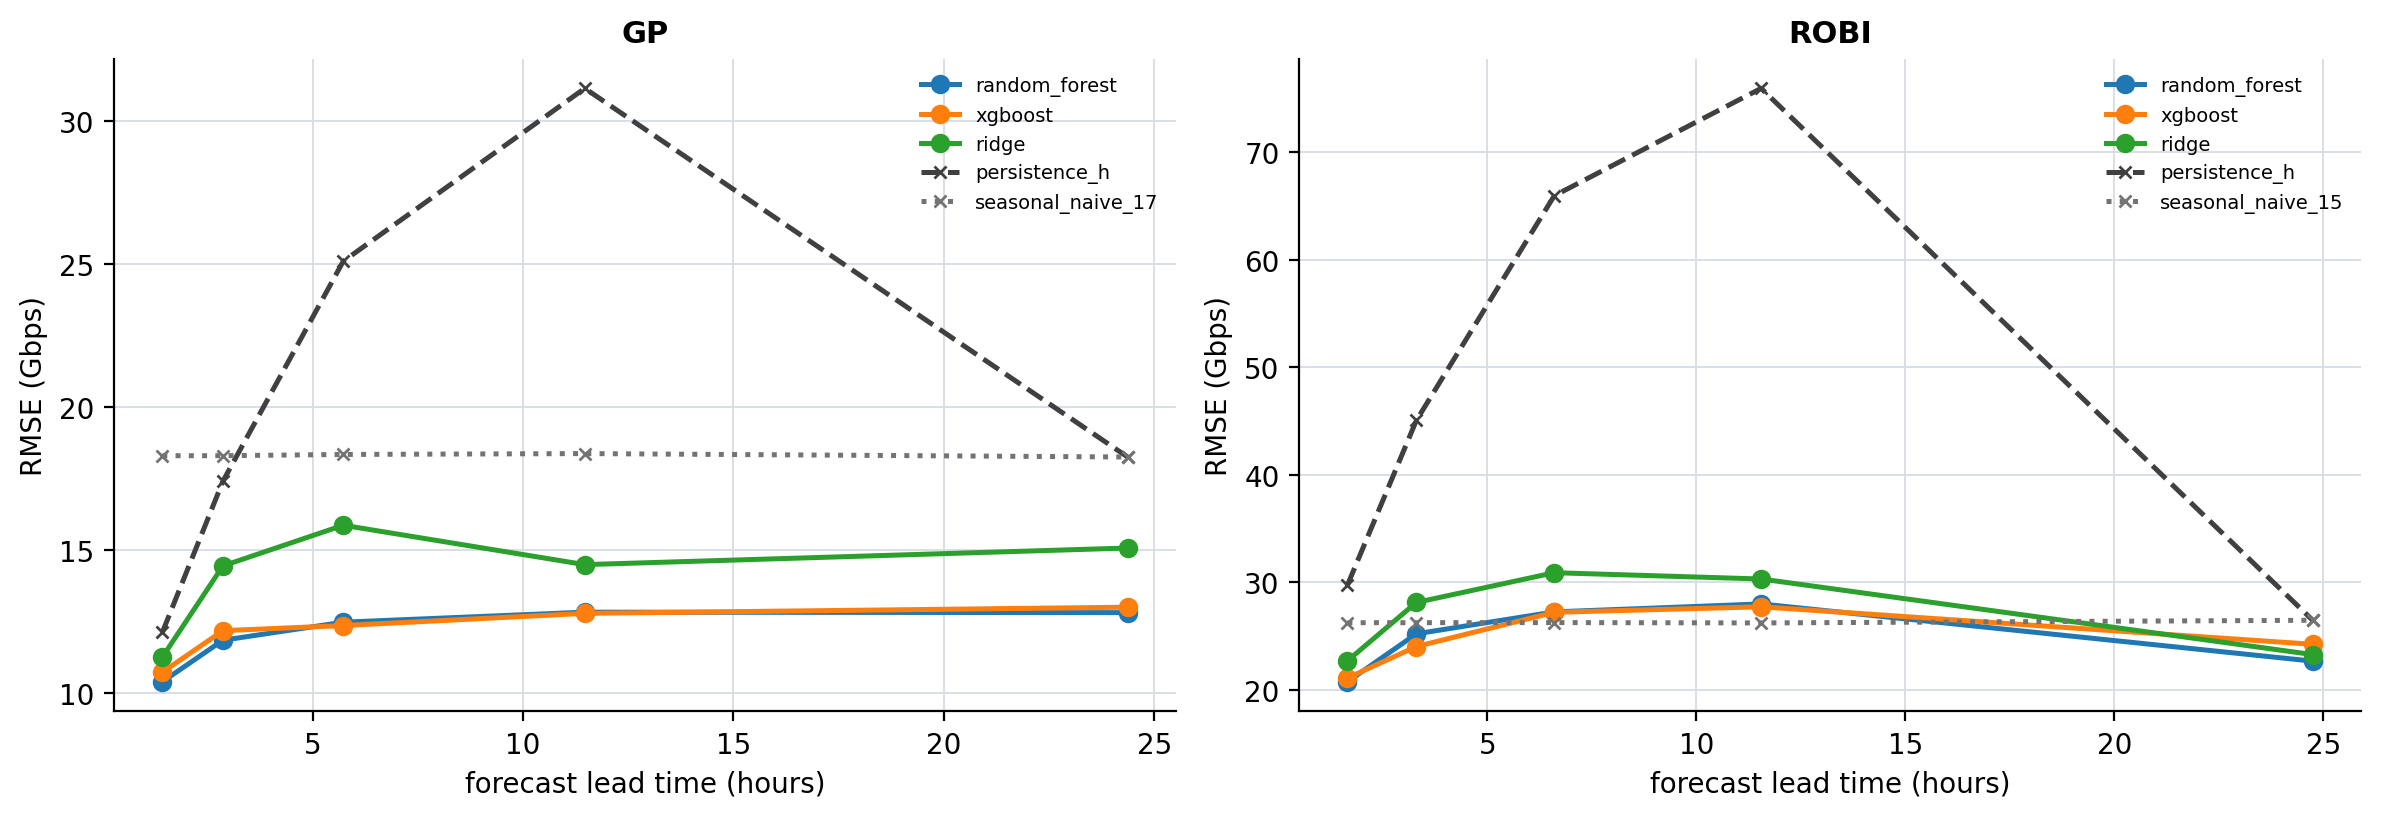
\includegraphics[width=\columnwidth]{fig5_horizon.png}
\caption{Accuracy against lead time, both operators. The learned model degrades far
more slowly than the naive forecaster at the same lead.}
\label{fig:horizon}
\end{figure}

\robix\ replicates it: $-30$\% at 1.65\,h growing to $-63$\% at 11.55\,h. Across a
$17\times$ longer horizon the learned model degrades 23\% while the naive baseline
degrades 157\%.

\textbf{This is the central empirical claim of the paper.} The value of learning on
these traces is not visible at one step; it is visible at the lead time an allocator
needs. The conventional one-step protocol measures these models in the single regime
where they look worst.

Two secondary findings follow. \emph{Direct beats recursive on \gpx} and the gap widens
with horizon (13.01 versus 24.18 at a 24-hour lead, $+86$\%); on \robix\ the two are
within noise at intermediate horizons, so the honest statement is that direct is the
safer default rather than a universal winner. And \emph{on \robix, forecasting 24 hours
ahead with yesterday's value at the same hour} (26.49) \emph{beats forecasting 1.6
hours ahead with the latest observation} (29.40). The daily cycle there is stronger
than short-run persistence. This inverts the usual decay-with-horizon intuition and is
visible only once the daily period is measured as 15 samples rather than assumed to be
24.

\section{Allocation}
\label{sec:alloc}

\subsection{Cost model}

For an allocation $A$ against realised demand $y$, with over-provisioning unit cost
$c_{o}$ and under-provisioning $\kappa$ times more expensive,
\begin{equation}
C = c_{o}\,(A-y)^{+} + \kappa\,c_{o}\,(y-A)^{+} .
\end{equation}
The cost-minimising allocation is the $\tau$-quantile of the predictive distribution
with
\begin{equation}
\tau^{*} = \frac{\kappa}{1+\kappa},
\end{equation}
so the operator's cost ratio \emph{selects the quantile}: $\kappa = 10$ gives
$\tau^{*} = 0.909$. We verify this correspondence empirically rather than only
asserting it.

\subsection{Calibration}

Quantile forecasts are calibrated by split conformal prediction, which is
distribution-free and finite-sample valid---the right choice at $n \approx 900$, where
no parametric error model is credible. An estimability guard refuses any $\tau$ a
calibration set cannot express (a set of $m$ residuals cannot express a level finer
than $1/(m+1)$; $\tau = 0.99$ needs 99) rather than silently returning the largest
residual.

\subsection{What to measure, and a comparison that does not work}
\label{sec:cost}

The natural comparison---capacity required at an equal SLA violation rate, against the
$A = 1.3\hat{y}$ rule operators use---\textbf{does not favour our method and we do not
claim it}. No conformal family reaches a 1\%, 2\% or 5\% violation target on either
trace. The reason is that the comparison is not well posed: drawing the fixed-margin
frontier requires knowing which margin achieved which violation rate \emph{on the test
data}, and ``the margin that lands at 1\% violations'' is a choice no operator can make
in advance. Conformal picks its level a priori from $\kappa$. Scoring an a-priori
method against a hindsight-tuned heuristic on the heuristic's home metric is not a fair
test. We also implemented a multiplicative conformal variant, on the hypothesis that an
additive-versus-multiplicative mismatch explained the gap; it did not ($-3.1$\% against
$-2.7$\%), which is what rules that explanation out.

\begin{table}[htbp]
\caption{Provisioning cost at $\kappa = 10$, against a fixed-margin rule given its best
hindsight-tuned margin---a setup biased against us.}
\label{tab:cost}
\centering
\begin{tabular}{lcc}
\toprule
\textbf{Method ($\kappa = 10$)} & \textbf{Cost at $\tau^{*}$} & \textbf{vs tuned} \\
\midrule
\gpx, context-adaptive & \textbf{19.27} & $\mathbf{-7.5\%}$ \\
\gpx, Mondrian & 20.11 & $-3.5$\% \\
\gpx, marginal & 21.35 & $+2.4$\% \emph{(worse)} \\
\gpx, fixed margin (tuned) & 20.84 & --- \\
\gpx, static peak & 29.52 & $+41.6$\% \emph{(worse)} \\
\midrule
\robix, context-adaptive & \textbf{49.34} & $\mathbf{-14.8\%}$ \\
\robix, marginal & 59.09 & $+2.0$\% \emph{(worse)} \\
\robix, fixed margin (tuned) & 57.93 & --- \\
\bottomrule
\end{tabular}
\end{table}

\begin{figure}[htbp]
\centering
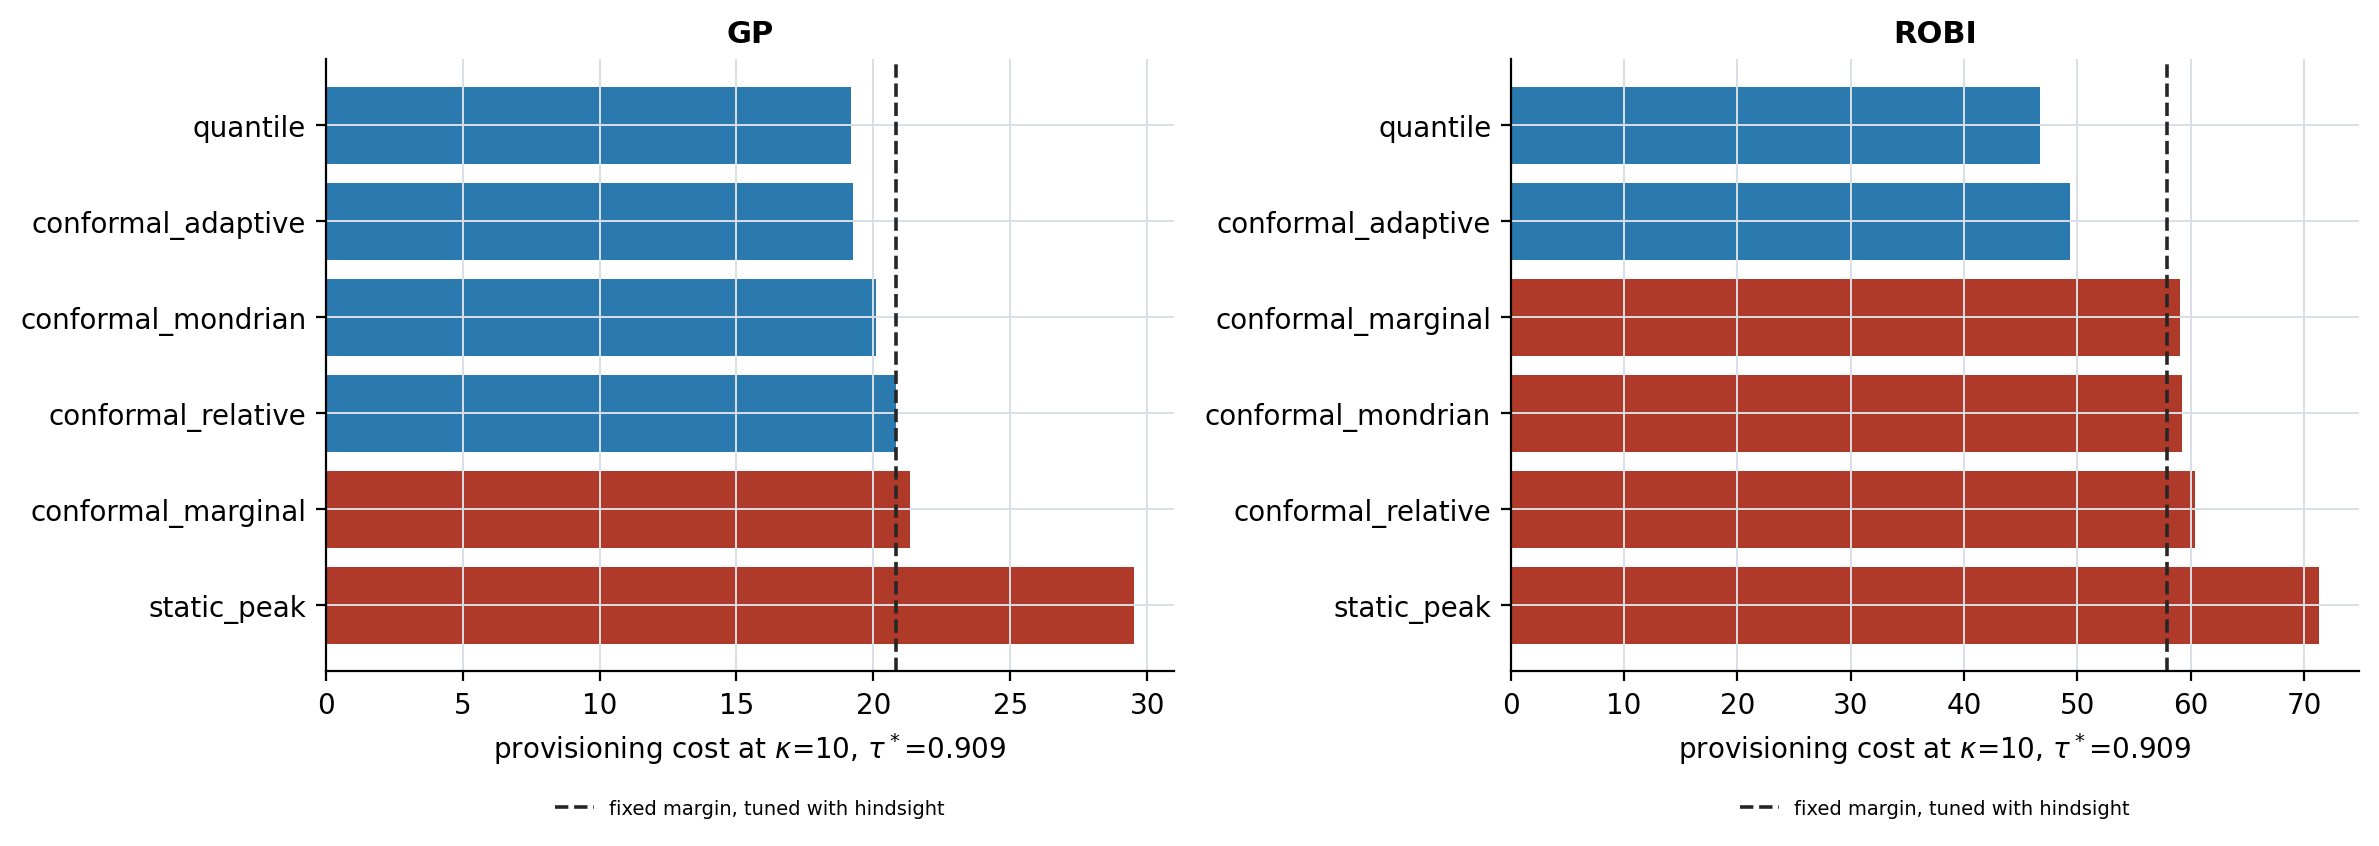
\includegraphics[width=\columnwidth]{fig7_cost.png}
\caption{Provisioning cost by calibration family, both operators.}
\label{fig:cost}
\end{figure}

Read the pattern, not the winner: \textbf{conditioning the margin on predicted
uncertainty beats the tuned heuristic on both operators; calibrating one margin for all
conditions loses to it on both.} That is Section~\ref{sec:context}'s idea, measured in
money.

\section{Context-Conditional Calibration}
\label{sec:context}

\subsection{Context acts on variance, not level}

Welch $t$-tests on the level and Levene tests on the spread of hour-detrended
residuals, \gpx:

\begin{table}[htbp]
\caption{Context-flag audit on \gpx. Six of nine flags are indistinguishable from noise
on the mean; one raises the residual spread by a third.}
\label{tab:flags}
\centering
\setlength{\tabcolsep}{4pt}
\begin{tabular}{lrrrrr}
\toprule
\textbf{Flag} & $n$ & $\Delta$\,mean & $p$\,(level) & $\sigma$ ratio & $p$\,(var.) \\
\midrule
\texttt{is\_weekend} & 261 & $+0.37$ & \textbf{0.77} & 0.96 & ns \\
\texttt{is\_event} & 275 & $-0.23$ & 0.86 & 1.02 & ns \\
\texttt{is\_drama} & 147 & $-1.52$ & 0.34 & 1.00 & ns \\
\texttt{is\_powercut} & 118 & $-2.63$ & 0.13 & 1.02 & ns \\
\texttt{is\_political} & 101 & $+2.69$ & 0.17 & 1.07 & ns \\
\textbf{\texttt{is\_rain}} & \textbf{131} & $+4.50$ & 0.026 & \textbf{1.330} & $\mathbf{<0.001}$ \\
\texttt{is\_offer} & 235 & $-5.73$ & 5.1e-06 & 0.90 & ns \\
\bottomrule
\end{tabular}
\end{table}

Two things follow. Six of the nine flags are indistinguishable from noise on the mean,
including the weekend flag that \textbf{both source filenames advertise}. And
\texttt{is\_rain} raises residual $\sigma$ from 16.4 to 21.8 Gbps---a 33\% increase in
\emph{uncertainty}---while moving the mean only modestly.

A point forecaster with a context dummy cannot express that. A context-conditional
prediction interval can. This converts weak mean-predictors into useful \textbf{risk}
signals: the flags need not predict demand well, only mark when the forecast is less
trustworthy.

\begin{figure}[htbp]
\centering
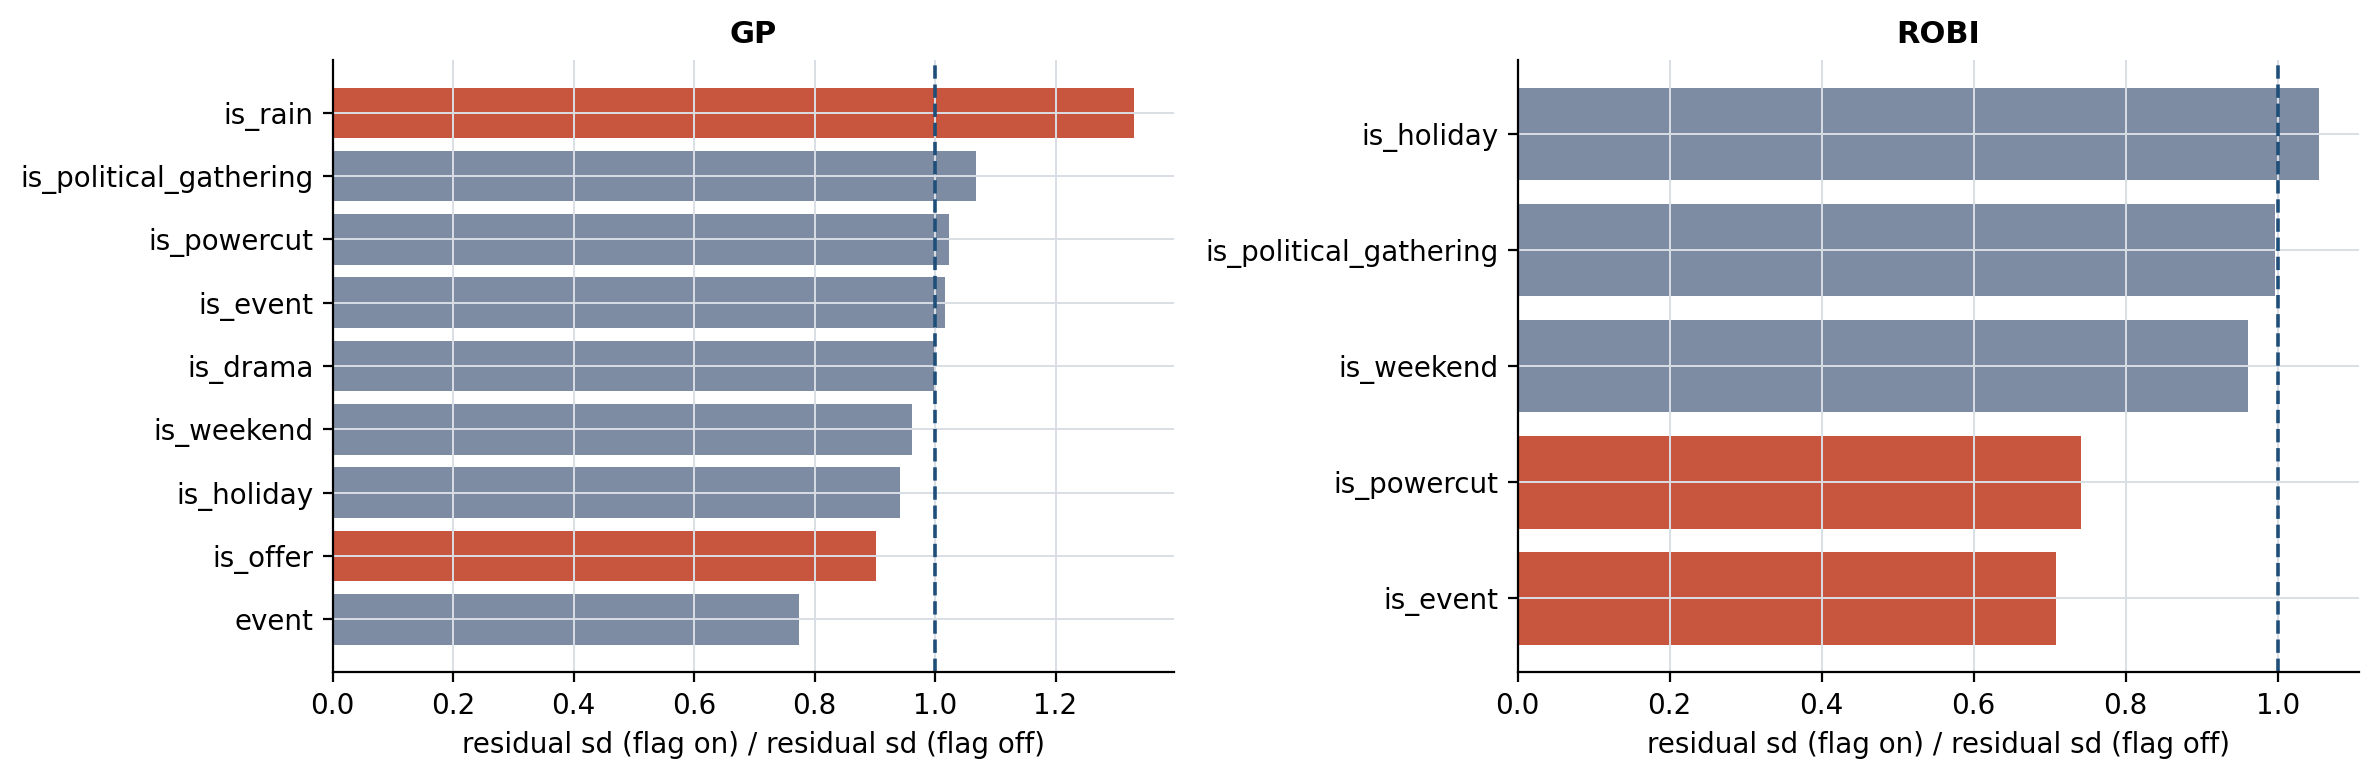
\includegraphics[width=\columnwidth]{fig6_flag_audit.png}
\caption{Context-flag audit: effect on level against effect on residual spread.}
\label{fig:flags}
\end{figure}

\subsection{The failure, and the repair}

Groups are formed by priority to keep them disjoint, and merged into two---%
\emph{elevated risk} $=$ rain $\cup$ gathering (199 rows) against \emph{baseline}
(689)---because a four-group split leaves the gathering group with $\sim$20 calibration
residuals. The baseline group carries $n = 354$ test points and the elevated-risk group
$n = 179$; exact Clopper--Pearson intervals are used rather than a normal
approximation, which at $n = 179$ is not reliable.

\begin{table*}[htbp]
\caption{\gpx: coverage pooled across folds, with Clopper--Pearson 95\% intervals. The
failure of marginal calibration inside the elevated-risk group is decisive; the
context-conditional repair is directional.}
\label{tab:coverage}
\centering
\begin{tabular}{llllll}
\toprule
\textbf{Nominal $\tau$} & \textbf{Group} & \textbf{Marginal} & \textbf{Locally adaptive} & \textbf{Mondrian} & \textbf{Online (ACI)} \\
\midrule
0.80 & baseline & 0.831 [.787, .868] & 0.814 [.769, .853] & 0.799 [.754, .840] & 0.825 [.781, .863] \\
0.80 & \textbf{elevated} & \textbf{0.693 [.620, .759]} & 0.726 [.655, .790] & 0.732 [.661, .795] & 0.760 [.690, .820] \\
0.90 & baseline & 0.915 [.881, .942] & 0.887 [.849, .918] & 0.887 [.849, .918] & 0.901 [.865, .930] \\
0.90 & \textbf{elevated} & \textbf{0.771 [.702, .830]} & 0.816 [.751, .870] & 0.788 [.720, .845] & \textbf{0.911 [.859, .948]} \\
0.95 & baseline & 0.958 [.931, .976] & 0.929 [.898, .954] & 0.944 [.914, .965] & 0.949 [.921, .970] \\
0.95 & \textbf{elevated} & \textbf{0.866 [.807, .912]} & 0.899 [.846, .939] & 0.933 [.886, .965] & 0.944 [.900, .973] \\
\bottomrule
\end{tabular}
\end{table*}

\textbf{The failure is established; the repair is directional.} These two halves of the
claim have different evidential status and we separate them.

\emph{The failure is decisive.} At $\tau = 0.90$ and $\tau = 0.95$ the marginal
interval inside the elevated-risk group excludes the nominal level ([.702,\,.830]
against 0.90; [.807,\,.912] against 0.95). A marginally calibrated allocator
demonstrably does not deliver its promised service level when the network is under
stress.

\emph{The context-conditional repair is not decisive at this sample size.} Locally
adaptive calibration moves the $\tau = 0.95$ elevated-risk estimate from 0.866 to
0.899, but the intervals overlap substantially and the adaptive interval still excludes
0.95. Mondrian does better (0.933, [.886,\,.965], which does contain the nominal level)
but on the same 179 points. The point estimates favour the context-conditional methods
at every level on both groups; the intervals do not separate them from marginal
calibration. This is a limit of the data, not of the method: 179 elevated-risk test
points cannot resolve a 3--7 point coverage difference.

\begin{figure}[htbp]
\centering
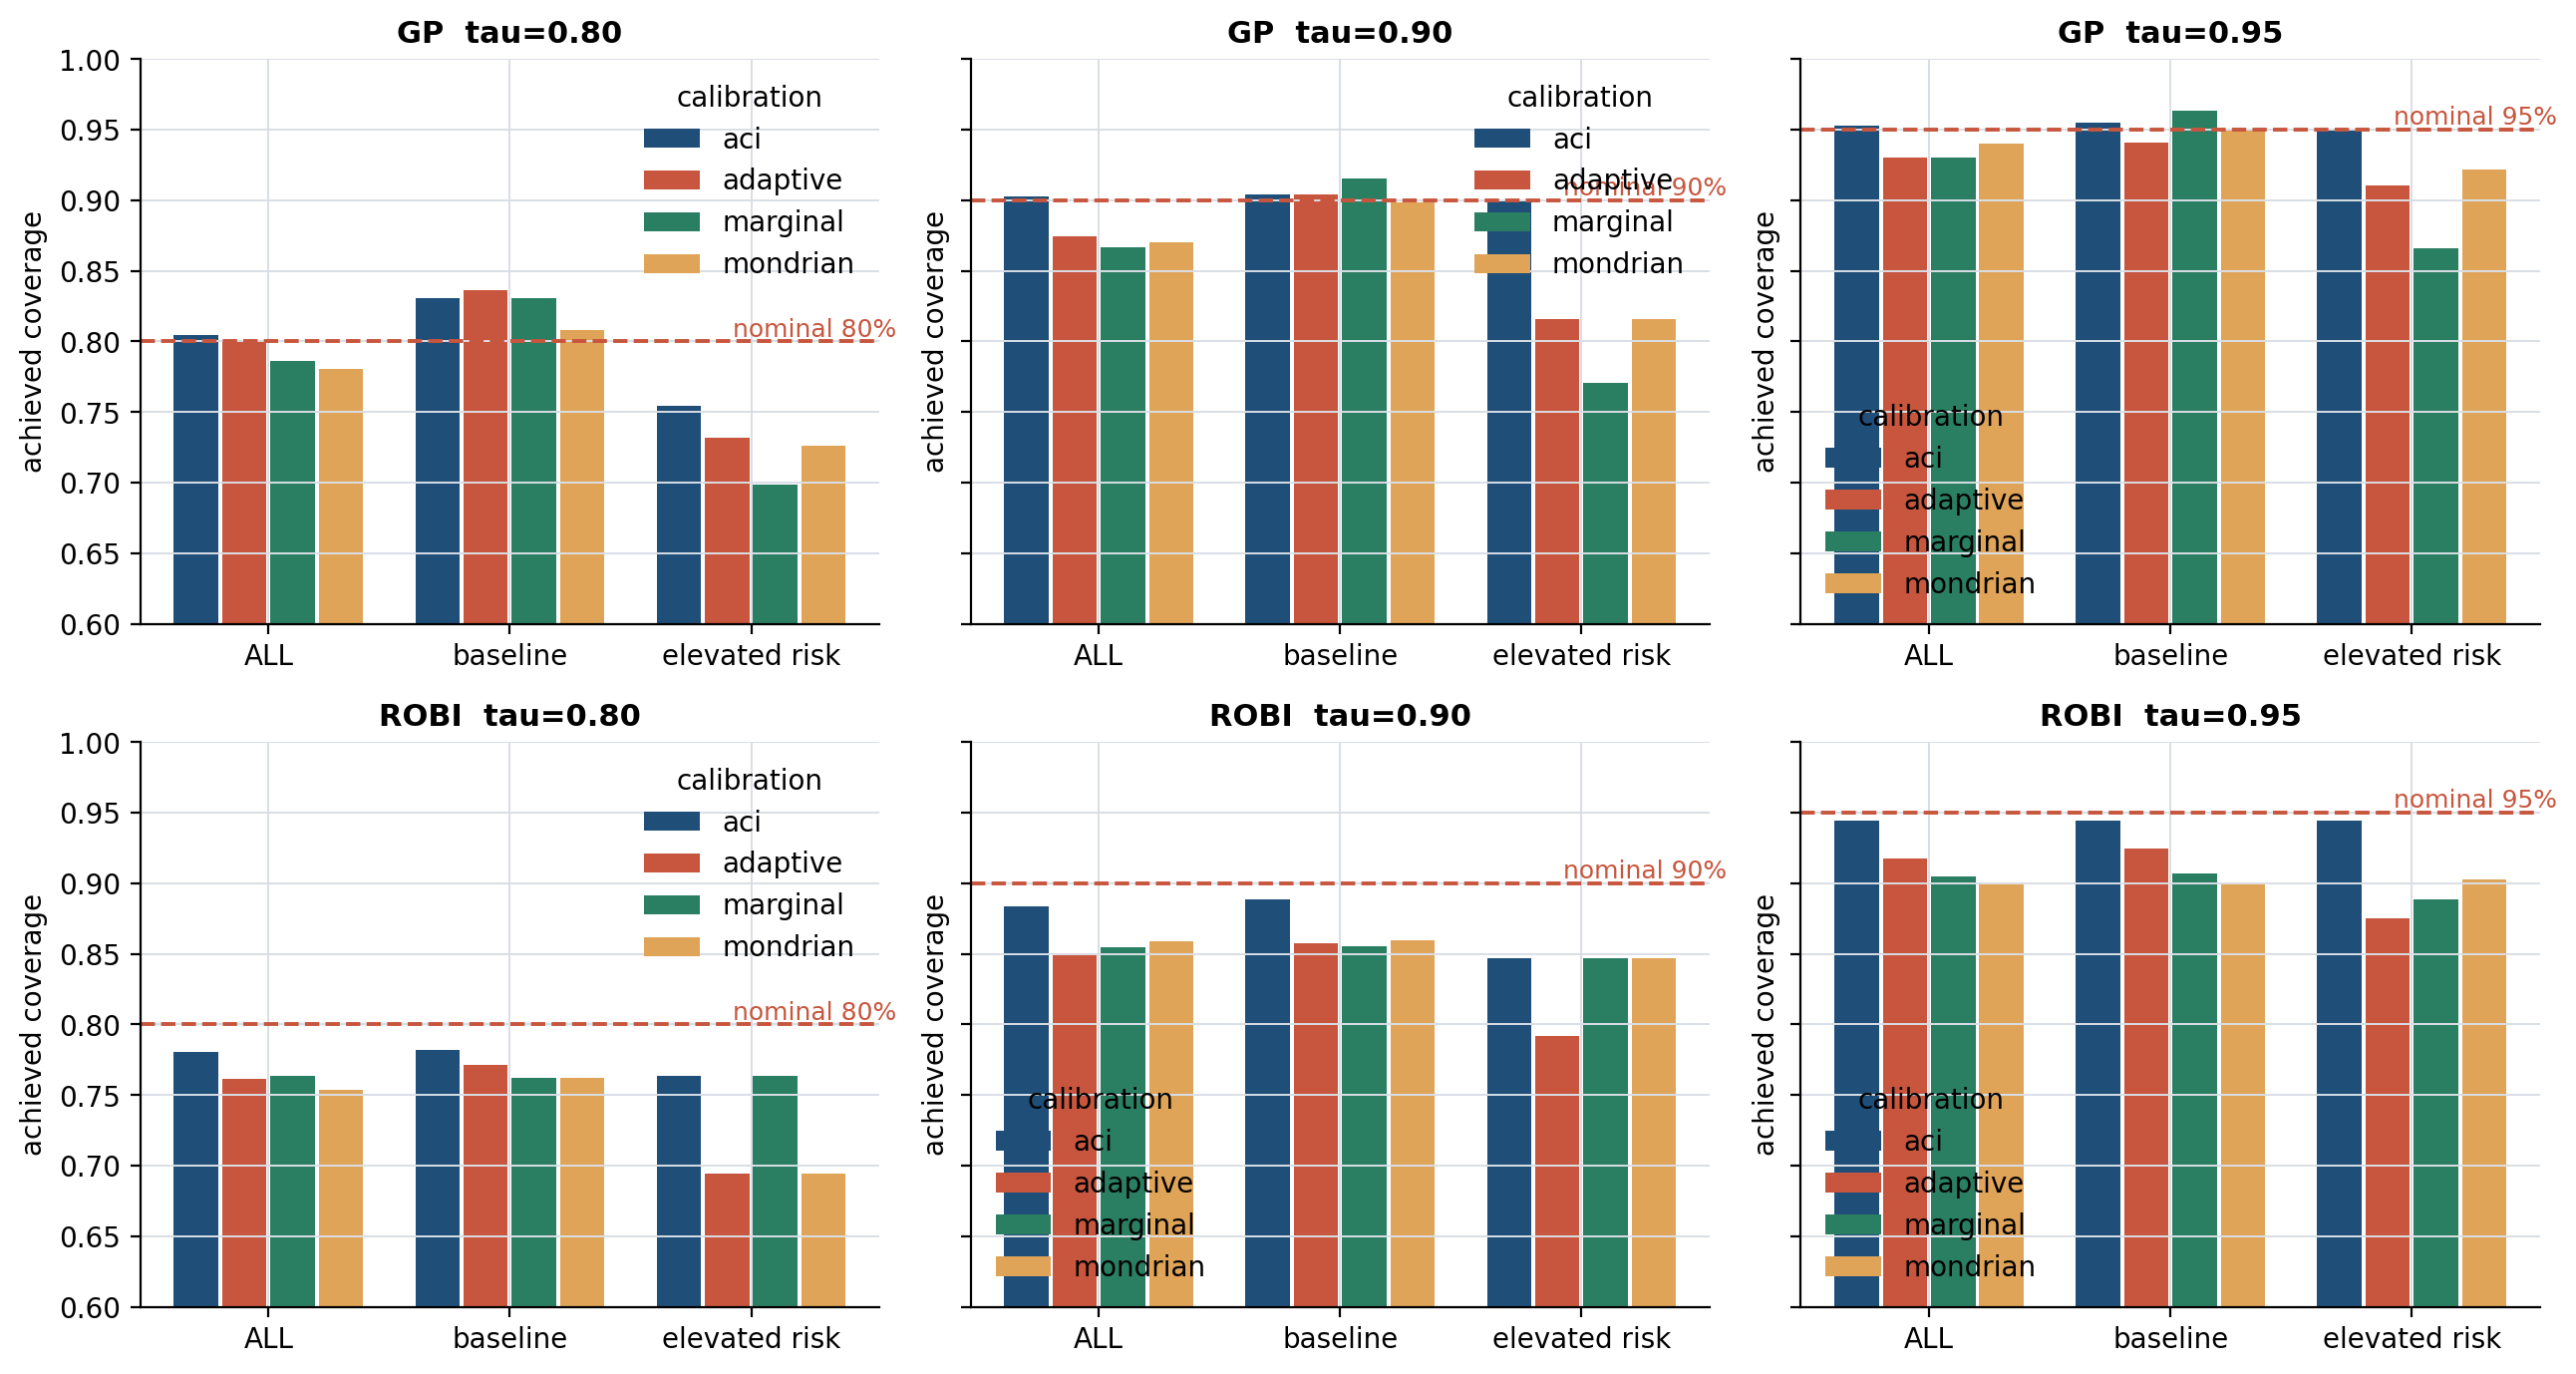
\includegraphics[width=\columnwidth]{fig4_coverage_by_group.png}
\caption{Per-context coverage, both operators, three levels.}
\label{fig:coverage}
\end{figure}

\textbf{An unexpected result.} The largest and only clearly decisive improvement inside
the elevated-risk group comes from \emph{online} calibration, which is not
context-conditional at all: at $\tau = 0.90$ it reaches 0.911 [.859,\,.948] against
marginal's 0.771 [.702,\,.830]---non-overlapping intervals. Adaptive conformal
inference adapts to \emph{whatever} is currently causing breaches, and elevated-risk
periods are clustered in time, so an online level update partly absorbs them without
ever being told the context. The honest reading is that the two mechanisms are
complementary and that on this dataset the temporal one is better evidenced than the
contextual one. A per-group online update---the obvious combination---is untried here
and is the clearest next step. The capacity cost of all of this is near-identical
($\sim 1.18\times$ demand at $\tau = 0.95$).

\subsection{The prediction is falsifiable, and it is null on Robi}

The audit finds \textbf{no \robix\ flag with elevated residual
variance}---\texttt{is\_powercut} and \texttt{is\_event} mark \emph{calmer}
periods---and \robix\ carries no rain annotation. The method should therefore do
nothing there, and it does: at $\tau = 0.95$ the elevated-risk group sees 0.889
(marginal), 0.875 (adaptive), 0.903 (Mondrian).

We state the claim in this form: \emph{context-conditional calibration helps exactly
when context carries variance signal, and whether it does can be tested in advance.} A
falsifiable prediction confirmed in both directions on two operators is stronger than
``it works''.

\subsection{A caveat on the cost result}

On \robix\ the adaptive cost gain of Section~\ref{sec:cost} cannot be credited to
context. The uncertainty model learns $\hat{\sigma}(x)$ from the whole feature vector,
so where no flag carries variance signal the adaptivity comes from time and lag
features. The supportable claim is that \emph{conditioning the margin on predicted
uncertainty pays}; only on \gpx\ is that uncertainty demonstrably contextual.

\section{Cold Start}
\label{sec:coldstart}

How much of its own history does a newly deployed site need? We run four arms on a
fixed \gpx\ test window with \robix\ as the source. This is possible only because
Section~\ref{sec:protocol} defines lags in wall-clock hours: at 86 and 99 min per
sample, a design matrix indexed by sample count is not comparable across sites.

\begin{table}[htbp]
\caption{Cold start at a 6-hour lead (persistence $=26.49$). RMSE by days of the new
site's own history.}
\label{tab:coldstart}
\centering
\setlength{\tabcolsep}{4pt}
\begin{tabular}{lccccc}
\toprule
\textbf{Days of local history} & 3 & 5 & 7 & 14 & 21 \\
\midrule
Own data alone & 20.61 & 19.81 & 18.98 & \textbf{14.82} & 15.86 \\
Pretrained $+$ fine-tuned & \textbf{19.65} & 19.87 & 19.91 & 15.63 & 17.45 \\
Pretrained, no fine-tuning & 20.39 & 20.01 & 19.74 & 19.06 & 19.04 \\
\bottomrule
\end{tabular}
\end{table}

\begin{figure}[htbp]
\centering
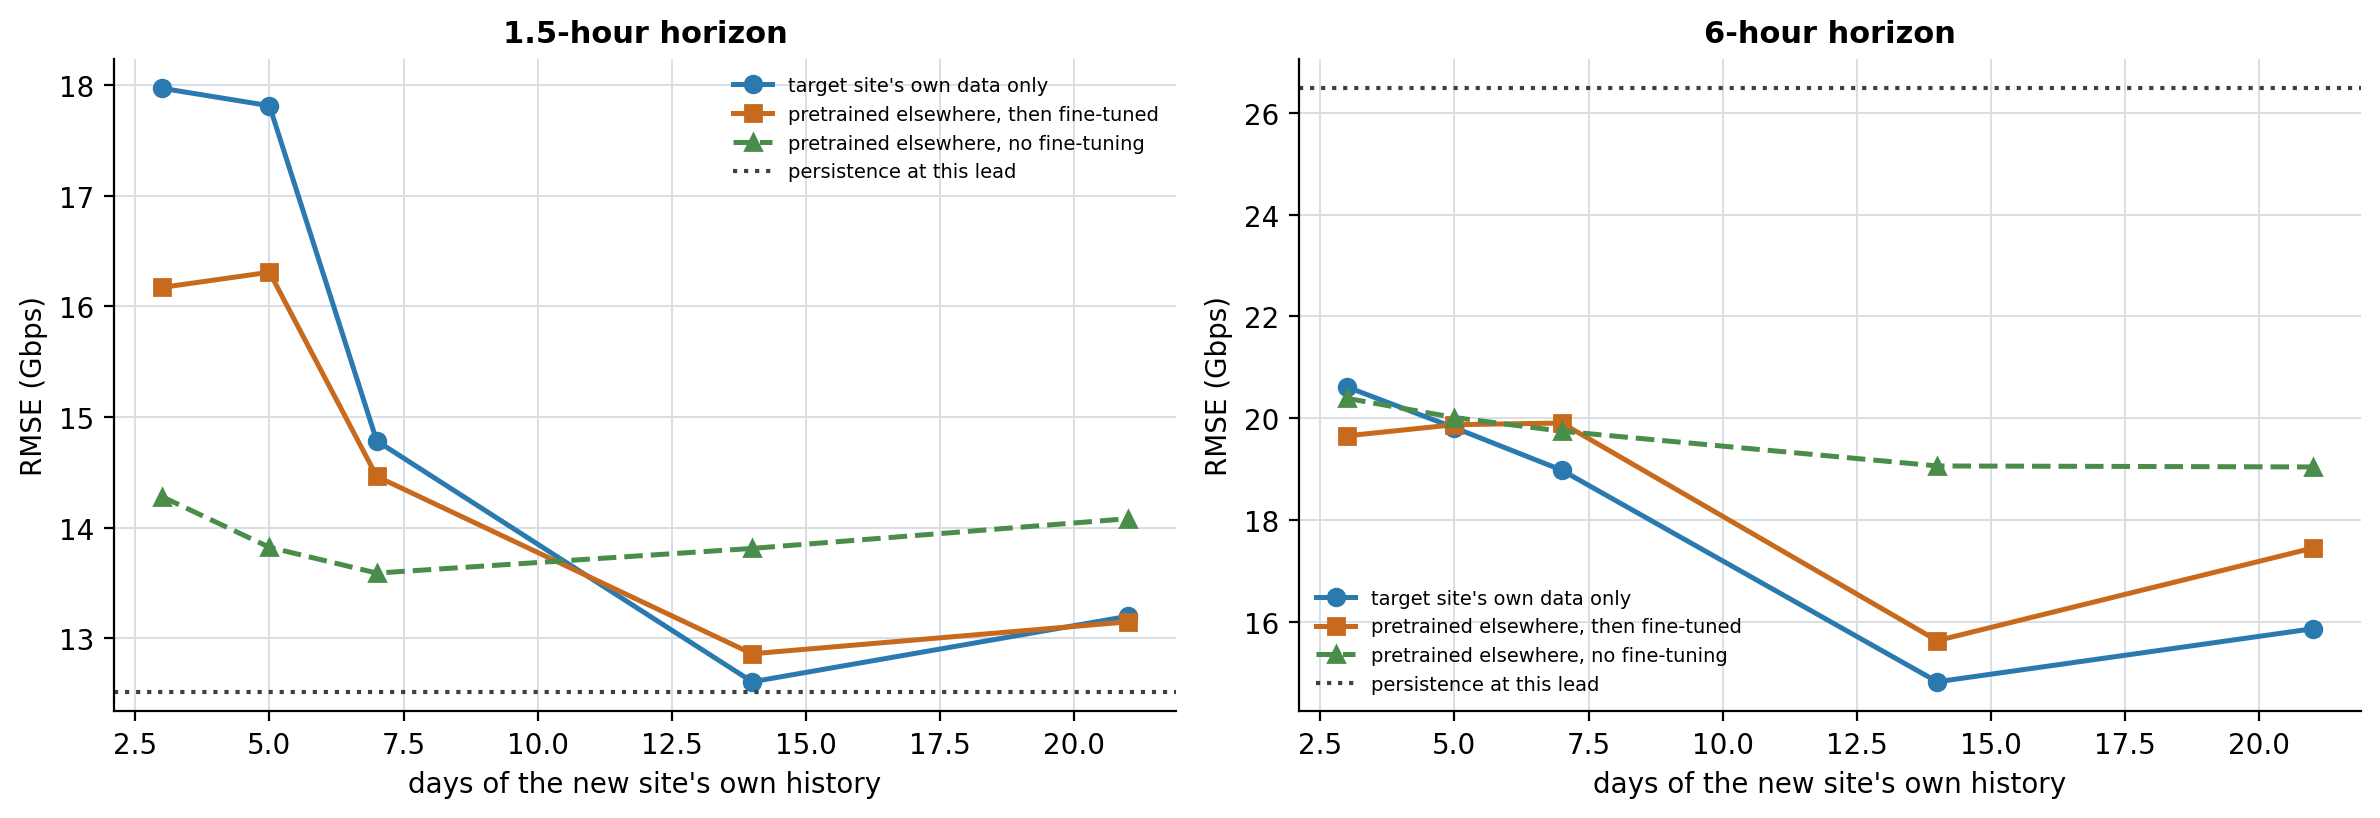
\includegraphics[width=\columnwidth]{fig8_transfer.png}
\caption{Cold-start curves at both horizons.}
\label{fig:transfer}
\end{figure}

A model trained entirely on the other operator, given only enough history to fix the
new site's level and scale, is 23\% better than persistence with \textbf{zero} training
data of its own. Pretraining then helps only while the site is data-poor: $+4.6$\% at 3
days, nothing by 5--7, and $-10$\% by 21 days where the borrowed weights hold the model
back. \textbf{The crossover is about a week.} At a 1.5-hour lead the study answers
nothing---no arm beats persistence---which is a second demonstration of
Section~\ref{sec:lead}.

\section{Zero-Shot Foundation Models}
\label{sec:zeroshot}

With $\sim$900 samples per site, is bespoke per-operator training worth it, or does a
model that has never seen this network do just as well? We evaluate Chronos-Bolt Small
strictly zero-shot---no fitting, no fine-tuning, not even a scaling constant---on the
same fold schedule, lead times and test blocks as Section~\ref{sec:lead}. It runs on
CPU in about seven minutes.

\subsection{The answer depends entirely on the operator}

\begin{table}[htbp]
\caption{Zero-shot Chronos-Bolt against the best trained model and against persistence.}
\label{tab:zeroshot}
\centering
\setlength{\tabcolsep}{4pt}
\begin{tabular}{lcccc}
\toprule
\textbf{Lead} & \textbf{Zero-shot} & \textbf{Best trained} & \textbf{vs trained} & \textbf{vs pers.} \\
\midrule
\multicolumn{5}{l}{\emph{\gpx}} \\
1.4\,h & 11.18 & 10.40 & $+7.5$\% & $-7.8$\% \\
2.9\,h & 13.53 & 11.85 & $+14.2$\% & $-22.3$\% \\
5.7\,h & 13.50 & 12.36 & $+9.2$\% & $-46.2$\% \\
11.5\,h & 14.41 & 12.79 & $+12.7$\% & $-53.8$\% \\
24.4\,h & 15.20 & 12.82 & $+18.6$\% & $-16.8$\% \\
\midrule
\multicolumn{5}{l}{\emph{\robix}} \\
1.7\,h & 30.54 & 20.77 & $+47.1$\% & $\mathbf{+2.7\%}$ \\
3.3\,h & 38.84 & 24.04 & $+61.5$\% & $-13.8$\% \\
6.6\,h & 40.34 & 27.23 & $+48.2$\% & $-38.8$\% \\
11.6\,h & 42.56 & 27.74 & $+53.4$\% & $-44.0$\% \\
24.8\,h & 43.63 & 22.69 & $\mathbf{+92.3\%}$ & $\mathbf{+64.7\%}$ \\
\bottomrule
\end{tabular}
\end{table}

On \gpx\ the zero-shot model is a credible system: it beats persistence at every lead,
by as much as 54\%, and trails a model trained on the site's own history by only
7.5--18.6\%. On \robix\ it trails by 47--92\% and is \emph{worse than persistence} at
both the shortest and the longest lead.

\begin{figure}[htbp]
\centering
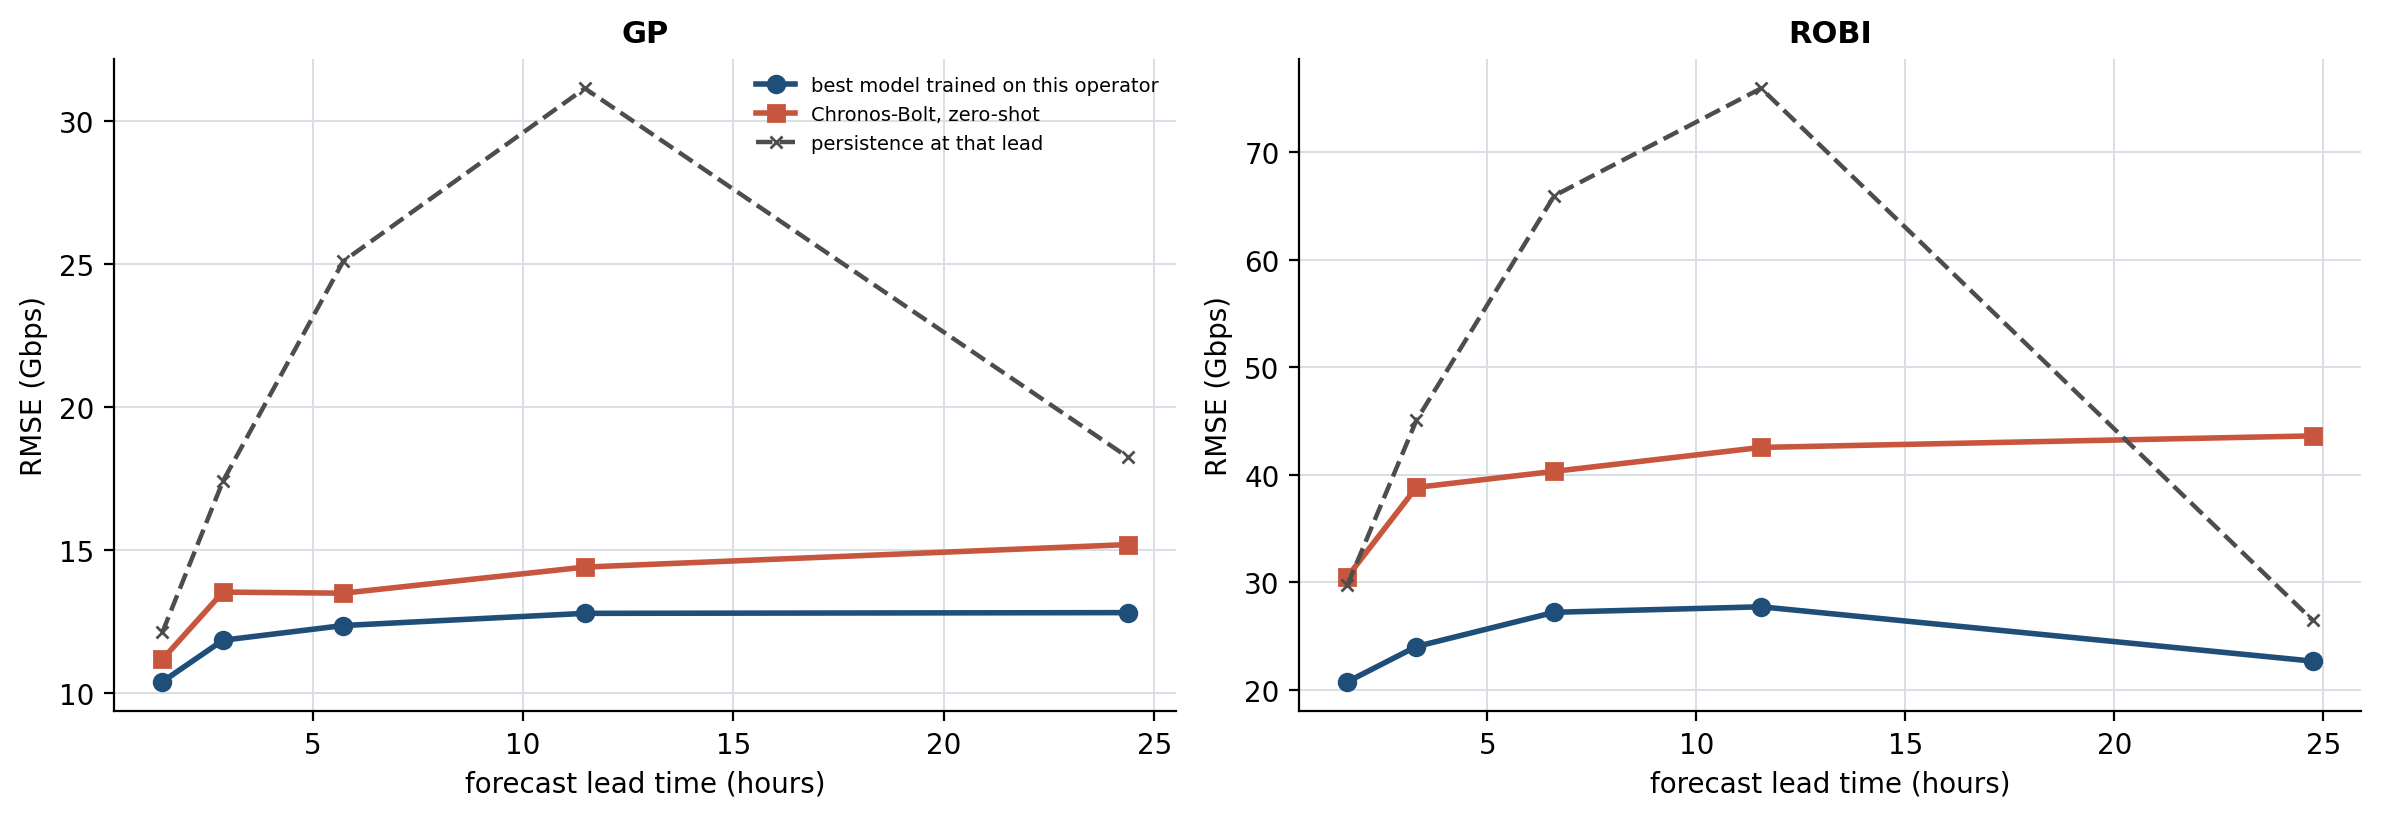
\includegraphics[width=\columnwidth]{fig9_foundation.png}
\caption{Zero-shot against trained and naive forecasters, both operators.}
\label{fig:foundation}
\end{figure}

\subsection{Why, and it is predictable in advance}

The gap is not random, and Section~\ref{sec:protocol} explains it. A foundation model
consumes a bare sequence of values with no timestamps. It cannot be told that a step is
86 minutes on one trace and 99 on the other, so it must infer periodicity from the
sequence itself---and on an irregularly sampled trace the daily cycle does not occupy a
whole number of steps.

\begin{table}[htbp]
\caption{Misregistration between the sampling grid and the daily cycle.}
\label{tab:misreg}
\centering
\begin{tabular}{lccc}
\toprule
& \textbf{Gap} & \textbf{Exact daily period} & \textbf{Drift/day} \\
\midrule
\gpx & 86 min & 16.744 samples & 0.256 \\
\robix & 99 min & \textbf{14.545 samples} & \textbf{0.455} \\
\bottomrule
\end{tabular}
\end{table}

\robix's cycle slips almost twice as fast. Over the 55-day span that is $\sim$25
samples of accumulated drift, about 1.7 complete cycles, against \gpx's $\sim$14. A
sequence model with no clock cannot hold phase against that, and the consequence is
exactly where theory says it should be: \textbf{the worst result of the entire
experiment is \robix\ at the 24-hour horizon} ($+92$\% against trained, $+65$\% against
persistence), the one setting where the daily cycle is the whole signal. The naive
baseline wins there simply by stepping back one \emph{measured} cycle---the thing the
foundation model cannot do.

This makes the sampling-rate correction more than a repair of prior work. It is a
\emph{diagnostic}: measuring the sampling interval tells an operator in advance whether
a timestamp-blind foundation model will work on their trace. We are not aware of this
being stated in the zero-shot forecasting literature, and it is cheap to check.

\subsection{Its quantiles cannot be used for provisioning as they come}

Chronos-Bolt is quantile-native, so it reaches the allocation layer with no
quantile-regression step. But its quantile head was trained on levels 0.1 to 0.9 only,
and a request above that is silently clipped---a $\tau = 0.95$ request returns the
$\tau = 0.90$ numbers unchanged. Since $\tau^{*} = \kappa/(1+\kappa)$, a ceiling of 0.9
corresponds to a cost asymmetry of only $\kappa = 9$. An operator for whom
under-provisioning costs $20\times$ more needs $\tau^{*} = 0.952$ and cannot obtain it
from the model at all.

\begin{table}[htbp]
\caption{Zero-shot quantile calibration, and its repair by split conformal.}
\label{tab:zsq}
\centering
\setlength{\tabcolsep}{4pt}
\begin{tabular}{llccc}
\toprule
\textbf{Op.} & $\tau$ & \textbf{Zero-shot} & \textbf{Conformalised} & \textbf{Capacity} \\
\midrule
\gpx & 0.80 & 0.791 & 0.815 & 1.112 $\rightarrow$ 1.124 \\
\gpx & 0.90 & 0.886 & 0.903 & 1.166 $\rightarrow$ 1.183 \\
\gpx & 0.95 & 0.886\,\emph{(clip)} & 0.941 & 1.166 $\rightarrow$ 1.225 \\
\robix & 0.80 & \textbf{0.662} & 0.813 & 1.148 $\rightarrow$ 1.245 \\
\robix & 0.90 & \textbf{0.786} & 0.909 & 1.230 $\rightarrow$ 1.328 \\
\robix & 0.95 & 0.786\,\emph{(clip)} & 0.950 & 1.230 $\rightarrow$ 1.389 \\
\bottomrule
\end{tabular}
\end{table}

On \robix\ the zero-shot 80\% interval delivers 66\%. Split-conformal calibration on
held-out residuals repairs every level on both traces, including the ones the model
cannot express natively. So the allocation machinery is not an alternative to the
foundation model; it is what makes the foundation model deployable. That is the useful
synthesis: \textbf{a zero-shot forecaster supplies the point prediction cheaply, and
conformal calibration supplies the service-level guarantee it cannot provide itself.}

\section{A Negative Result on Coverage, and Its Repair}
\label{sec:cov}

Enforcing the $\pm 2\%$ coverage check on real backtest output rather than synthetic
data: \textbf{249 of 360 configurations fail, 232 of them by under-covering; of the 30
marginal configurations, only 2 pass.} The one-sidedness is diagnostic. Split
conformal's guarantee is conditional on exchangeability, and a 55-day trace with a
trend does not supply it.

We therefore apply adaptive conformal inference, updating the requested miscoverage
online from realised breaches,
\begin{equation}
\alpha \leftarrow \alpha + \gamma\,(\alpha_{\mathrm{target}} - \mathrm{err}),
\end{equation}
whose long-run coverage converges without any exchangeability assumption. All feedback
is strictly causal: the outcome at $t$ affects only allocations from $t+1$.

\begin{table}[htbp]
\caption{Marginal coverage across 5 lead times, 3 levels and both operators---30
configurations.}
\label{tab:aci}
\centering
\begin{tabular}{lccc}
\toprule
\textbf{Method} & \textbf{Passing $\pm 2\%$} & \textbf{\gpx\ gap} & \textbf{\robix\ gap} \\
\midrule
\textbf{Online (ACI)} & \textbf{30 / 30} & \textbf{$+0.2$ pp} & \textbf{$-0.9$ pp} \\
Locally adaptive & 6 / 30 & $-2.8$ pp & $-4.2$ pp \\
Mondrian & 5 / 30 & $-3.3$ pp & $-5.5$ pp \\
Marginal & 2 / 30 & $-3.4$ pp & $-4.9$ pp \\
\bottomrule
\end{tabular}
\end{table}

\begin{table}[htbp]
\caption{\gpx: achieved coverage by lead time. Online calibration holds its target as
the forecast degrades; static calibration does not.}
\label{tab:acilead}
\centering
\setlength{\tabcolsep}{4pt}
\begin{tabular}{lccccc}
\toprule
$\tau$ & 1.4\,h & 2.9\,h & 5.7\,h & 11.5\,h & 24.4\,h \\
\midrule
0.90, online & 0.904 & 0.902 & 0.906 & 0.907 & 0.901 \\
0.90, marginal & 0.867 & 0.878 & 0.851 & 0.839 & 0.868 \\
0.95, online & 0.947 & 0.946 & 0.949 & 0.945 & 0.950 \\
0.95, marginal & 0.927 & 0.957 & 0.915 & 0.909 & 0.924 \\
\bottomrule
\end{tabular}
\end{table}

\textbf{Online calibration holds its nominal service level in all 30 (operator, lead
time, level) configurations, while static calibration meets it in 2 to 6 and drifts as
far as 7 points below nominal as the forecast degrades.} For a deployable allocator
this is the property that matters.

This is \emph{marginal} coverage, and we do not overstate it: counting per-group rows
as well, ACI passes 61 of 90 configurations against 12--20 for the static methods. ACI
is not group-conditional, so it does not subsume Section~\ref{sec:context}---the two
repairs address different failures and are complementary. A per-group online update is
the obvious next step and is untried here.

\section{Limitations}

905 and 888 observations from two cell sites over $\sim$2 months. The sample size does
not support strong claims about model superiority, and the span cannot speak to
seasonal or annual effects. Context flags are hand-labelled by a single annotator with
no inter-rater check. \robix\ carries five of the nine flags and no rain annotation, so
its context-conditional results rest on an 89-row group and are directional only.

Two limits are measured rather than asserted, and both are reported above: correcting
the feature design does not improve accuracy (Section~\ref{sec:ablation}), and
split-conformal coverage fails its $\pm 2\%$ target on these traces
(Section~\ref{sec:cov}). Absolute coverage guarantees should not be claimed from the
static conformal results; the context-conditional comparison is unaffected, being a
relative comparison between methods calibrated on identical data.

The methods here are chosen to be robust to those limits rather than to hide them:
conformal calibration is distribution-free and finite-sample valid, the estimability
guard makes the sample-size ceiling explicit, and the drift that breaks exchangeability
is handled by a method that does not assume it.

\section{Conclusion}

Treating capacity planning as a forecasting problem scored by RMSE gets three things
wrong at once, and correcting each changes what the data says.

Correcting the \textbf{horizon} rescues the case for learning. At one step a learned
model beats persistence by 14\% on \gpx, a margin that would not justify deploying
anything; at the lead time a provisioning decision actually requires, it beats the
naive forecaster at that same lead by 59\%, and by 63\% on the second operator. The
conventional protocol measures these systems in the one regime where they look worst.

Correcting the \textbf{objective} makes the comparison meaningful. Scored on
provisioning cost at the level the theory prescribes from the operator's own cost
ratio---against a fixed-margin heuristic given its best margin with
hindsight---context-adaptive conformal allocation is 7.5\% (\gpx) and 14.8\% (\robix)
cheaper, while marginally calibrated allocation is \emph{worse} than that heuristic on
both traces. The saving comes specifically from conditioning the margin on predicted
uncertainty.

Correcting the \textbf{sampling assumption} is what makes anything comparable across
sites, and it pays two unanticipated dividends. Because lags are defined in wall-clock
hours rather than sample counts, a model trained on one operator transfers to the
other: given only enough history to fix a new site's scale, a borrowed model is 23\%
better than persistence with zero training data of its own, and the crossover to
training locally arrives after about a week. And the same measurement turns out to
\emph{predict} when a zero-shot foundation model will fail---such a model reads a bare
sequence with no clock, so it cannot hold phase against a daily cycle that occupies
14.545 samples, and it duly collapses on the trace where that misregistration is worst
while remaining competitive on the trace where it is not.

On the context-conditional claim we are deliberately careful. That marginal calibration
\emph{fails} inside high-variance contexts is established: at $\tau = 0.95$ its
elevated-risk interval is [.807,\,.912], excluding the nominal level. That
context-conditional calibration \emph{repairs} it is directional---the point estimates
improve at every level, but 179 elevated-risk test points cannot resolve a 3--7 point
difference. The largest decisive improvement on that group in fact comes from online
calibration, which is not context-conditional at all, because elevated-risk periods
cluster in time. A per-group online update is the obvious combination and is untried.

Two negative results are reported in full because they discipline the claims: the
corrected feature design does not improve RMSE, since tree ensembles route around a
mis-specified lag; and static conformal coverage fails its $\pm 2\%$ target almost
everywhere, because a 55-day trace with a trend does not satisfy exchangeability.
Online calibration repairs the latter completely---30 of 30 configurations---and that
is the property a deployable allocator needs.

None of this depends on the dataset being large, which is what makes it defensible at
$n = 900$. What the sample size does foreclose is any strong claim about model
superiority, and we make none.

\section*{Reproducibility}

Fixed seeds throughout. 47 verification gates encode the specific failures corrected
here---leakage, the sampling-rate assumption, the inverted split, the estimability
bound, the multi-horizon embargo, the causality of the online update---so a refactor
cannot silently reintroduce them. Every figure is regenerated from the stored result
tables alone, so the paper rebuilds without refitting any model.

\bibliographystyle{IEEEtran}
\bibliography{refs}

\end{document}
